\section{Generating Correlated Poisson Variables}\label{ch:generate_correlated_poisson}
In presenting the simulation procedure, it is necessary to discuss the method for generating correlated Poisson variables. The goal is to generate a $d$-dimensional multivariate random variable $\boldsymbol{X} = (x_1, x_2, \ldots, x_d)$ with mean $(\lambda_1, \lambda_2, \ldots, \lambda_{d})$ and $d$ x $d$ correlation matrix $R_d$ where each $X_i$ has a marginal distribution that is the same as the distribution of a Poisson variable with mean $\lambda_i$. That is, $P(X_i = x_i) = f_i(x_i)$, where $f_i$ is the probability mass function of a Poisson variable with mean $\lambda_i$. \cite{A8} describe a procedure for generating $\boldsymbol{X}$ using the copula approach. 

A copula is defined as any joint probability cumulative distribution function where each marginal distribution is uniformly distributed (\cite{B1}). That is, 

$$C(\boldsymbol{u}): [0,1]^d \to [0,1]$$ 

is a copula if $C(0, 0, \ldots, 0) = 0$ and $C(1, \ldots, 1, u_i, 1, \ldots, 1) = u_i$ and $u_i \in [0,1]$ for all $i$. The Gaussian copula as described in \cite{A8} is used, where

$$ C_R^{Gaussian}(u_1, u_2, \ldots, u_d) = \Phi_{R_d}(\Phi^{-1}(u_1), \Phi^{-1}(u_2), \ldots,  \Phi^{-1}(u_d))$$

in which $\Phi$ is the cumulative distribution function for a standard random normal variable and $\Phi_{R_d}$ is the cumulative distribution function for a multivariate normal random variable with mean $\boldsymbol{0}$, variance $\boldsymbol{1}$, and correlation matrix $R_d$. $\boldsymbol{u}$ can be generated by first generating a random multivariate normal variable $\boldsymbol{Y} = (y_1,y_2, \ldots, y_d)$ with correlation matrix $R_d$ and setting $(u_1, u_2, \ldots, u_d) = (\Phi(y_1), \Phi(y_2), \ldots,  \Phi(y_d))$. It can then be paired with a copula that has marginal Poisson distributions. Namely,

$$ C^{Poisson}(F_1(x_1), F_2(x_2), \ldots, F_d(x_d))$$ where $F_i$ is the discrete cumulative distribution function for a Poisson random variable with rate $\lambda_i$. $\boldsymbol{x}$ can then be set to

$$(x_1, x_2, \ldots, x_d) = (F^{-1}_1(u_1), F^{-1}_2(u_2), \ldots, F^{-1}_d(u_d))$$

To implement $F^{-1}_i(u_i)$, the inverse transform method as described in \cite{B1} is used:
$$ $$

\begin{algorithm}[H]
\SetAlgoLined
\caption{Inverse Transform Method for Generating a Poisson Rate Variable With Mean $\lambda$ and quantile $u$}
 Let $i = 0$ \;
 Let $p = e^{-\lambda}$ \;
 Let $F = p$ \;
 \While{$u \geq F$}{
  $p \leftarrow \lambda p / (i + 1)$ \;
  $F \leftarrow F + p$ \;
  $i \leftarrow i + 1$ \;
 }
 return $i$ \;
\end{algorithm}

Each $x_i$ will have a marginal Poisson distribution with rate $\lambda_i$ and $\boldsymbol{x}$ will approximately have correlation matrix $R_d$. Table \ref{tab:experimental_correlation} shows the accuracy of this method for different desired correlations using simulation. For each desired correlation, 10000 pairs of random variables $(x_1,x_2)$ are generated that have means $1$ and joint Poisson distribution (see Listing \ref{correlated-poisson}). For each correlation level, $x_1$ and $x_2$ have the correct means that are very near 1. For positive correlations, the actual correlation is slightly below the desired correlation (less than 0.1 difference at each desired correlation). For negative correlations, the actual correlation is slightly above the desired correlation for smaller magnitudes and deviates significantly at higher magnitudes. In practice, our correlation matrix $R$ contains values that range from small negative correlations to large positive correlations (see Tables \ref{fig:pos_pos_corr_pic}, \ref{fig:pos_neg_corr_pic}, and \ref{fig:neg_neg_corr_pic}), so this method would generate Poisson arrivals that follow $R$ closely. It may be possible to generate arrivals that more accurately reflect the given correlations, but this method provides acceptable performance for the given data.

\begin{table}
\label{tab:experimental_correlation}
\centering
\caption{Actual vs. Desired Correlation Using Gaussian Copula, $n=10000$}
\begin{tabular}{l|l|l|l}
\hline \hline
\textbf{Desired Correlation} & $\bar{x_1}$ & $\bar{x_2}$ & \textbf{Actual Correlation}  \\ 
\hline
-1                  & 0.995                           & 1.009                           & -0.735              \\
-0.9                & 0.997                           & 0.997                           & -0.682              \\
-0.8                & 1.010                            & 0.985                           & -0.616              \\
-0.7                & 0.987                           & 1.003                           & -0.543              \\
-0.6                & 0.990                            & 1.014                           & -0.472              \\
-0.5                & 0.998                           & 1.002                           & -0.405              \\
-0.4                & 1.016                           & 0.988                           & -0.308              \\
-0.3                & 1.003                           & 1.005                           & -0.236              \\
-0.2                & 1.001                           & 1.007                           & -0.163              \\
-0.1                & 0.998                           & 1.018                           & -0.086              \\
0                   & 1.014                           & 0.986                           & 0.016               \\
0.1                 & 0.976                           & 0.992                           & 0.062               \\
0.2                 & 0.994                           & 0.986                           & 0.162               \\
0.3                 & 0.995                           & 1.002                           & 0.246               \\
0.4                 & 1.006                           & 1.004                           & 0.371               \\
0.5                 & 1.000                               & 0.997                           & 0.433               \\
0.6                 & 0.987                           & 1.001                           & 0.522               \\
0.7                 & 1.007                           & 1.007                           & 0.616               \\
0.8                 & 0.993                           & 0.986                           & 0.727               \\
0.9                 & 1.010                            & 1.008                           & 0.829               \\
1                   & 0.997                           & 0.997                           & 1.000                  
\end{tabular}
\end{table}

\section{Backwards Simulation} \label{ch:backwards_simulation}

Using the methods in Section \ref{ch:generate_correlated_poisson}, the numbers of positive and negative events in a time period of length $t$ can be generated with means equal to $\lambda^{\pm}_k \cdot t$ and correlation matrix $R$. Given the numbers of arrivals, a method called backwards simulation can be used to simulate the times of events (\cite{A7}). 

Backwards simulation uses the fact that conditioned on the number of arrivals in a Poisson process during a time period $t$ being equal to $n$, these arrivals are distributed uniformly across $[0,t)$. Using this method, arrivals over a larger time period $T$ (i.e. $T = 10t$) can be generated by simulating arrivals in smaller chunks of size $t$. An algorithm is presented below for simulating arrivals over a time period $[s,s+t)$, with the arrivals following a $4K$-dimensional multivariate Poisson process with means $\lambda^{\pm}_k$ and correlation matrix $R$. The event sizes are distributed exponentially with means $\mu^{\pm}_k$ as described in Section \ref{ch:poisson}. It returns a list of events $E$ whose entries $(k,y,\tau)$ consist of the event position, size, and time respectively:
$$ $$

\begin{algorithm}[H]
\label{alg:backwards_simulation}
\SetAlgoLined
\caption{Backwards Simulation Method For Generating Correlated Poisson Arrivals During Time Period $[s, s+t)$}
 $E = []$;

 Generate Poisson variables $(n^{\pm}_{-K}, \ldots, n^{\pm}_{-1}, n^{\pm}_1, \ldots, n^{\pm}_K)$ with means $(\lambda^{\pm}_{-K}, \ldots, \lambda^{\pm}_{-1}, \lambda^{\pm}_1, \ldots, \lambda^{\pm}_K)$ and correlation matrix $R$ (see Section \ref{ch:generate_correlated_poisson}) \;
 
 \For{$k = -K, \ldots, -1, 1, \ldots, K$} {
    \For{$i = 1, \ldots, n^+_k$} {
        Generate $\tau$ $\sim$ Uniform($s$, $s+t$) \;
        Generate $y$ $\sim$ Exponential($\mu^+_k$) \;
        Append $(k,y,\tau)$ to $E$ \;
    }
    \For{$i = 1, \ldots, n^-_k$} {
        Generate $\tau$ $\sim$ Uniform($s$, $s+t$) \;
        Generate $y$ $\sim$ Exponential($\mu^-_k$) \;
        Append $(k,-y,\tau)$ to $E$ \;
    }
 }
 
 Return $E$ \;
 
\end{algorithm}

$$ $$

Sample arrivals using parameters estimated in Chapter \ref{ch:experiment} are shown in Figures \ref{fig:bid_events_graphs} and \ref{fig:ask_events_graphs}. Positive events are shown in blue while negative events are shown in orange.

\begin{figure}
\centering
\caption{Bid Arrivals over $T$ = 600 seconds}
\begin{tabular}{cc}
\hline
\subf{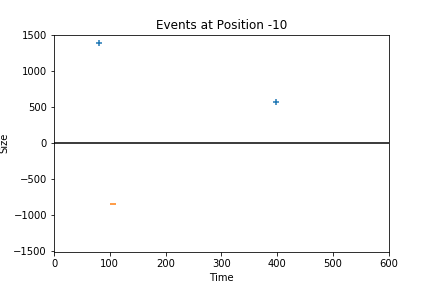
\includegraphics[width=60mm]{Figures/Events/events-10.png}}
{}
&
\subf{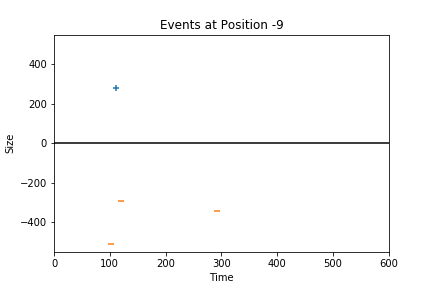
\includegraphics[width=60mm]{Figures/Events/events-9.png}}
{}
\\
\subf{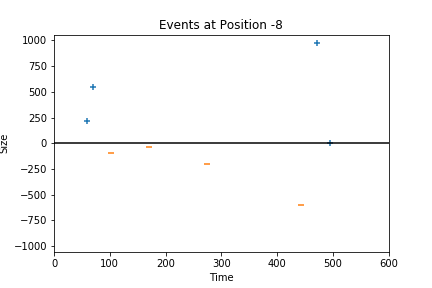
\includegraphics[width=60mm]{Figures/Events/events-8.png}}
{}
&
\subf{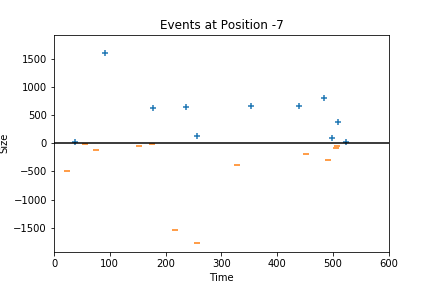
\includegraphics[width=60mm]{Figures/Events/events-7.png}}
{}
\\
\subf{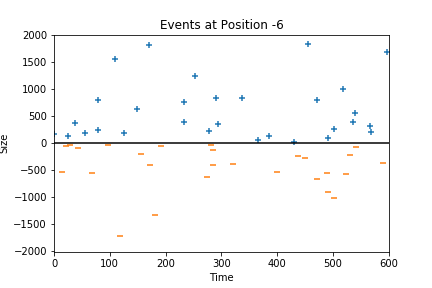
\includegraphics[width=60mm]{Figures/Events/events-6.png}}
{}
&
\subf{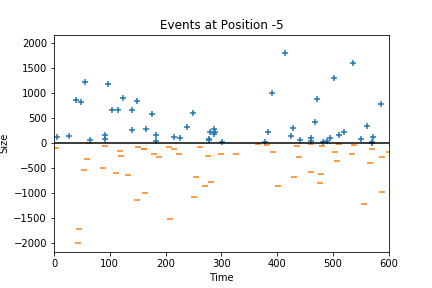
\includegraphics[width=60mm]{Figures/Events/events-5.png}}
{}
\\
\subf{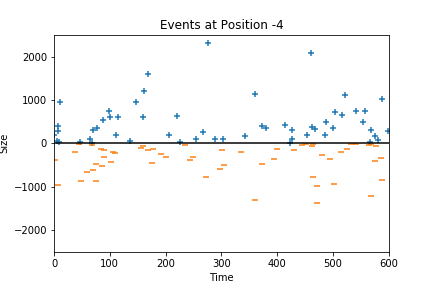
\includegraphics[width=60mm]{Figures/Events/events-4.png}}
{}
&
\subf{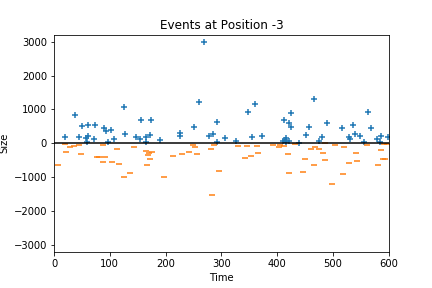
\includegraphics[width=60mm]{Figures/Events/events-3.png}}
{}
\\
\subf{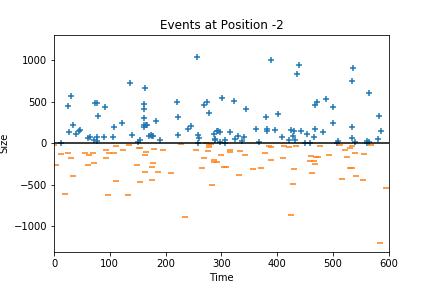
\includegraphics[width=60mm]{Figures/Events/events-2.png}}
{}
&
\subf{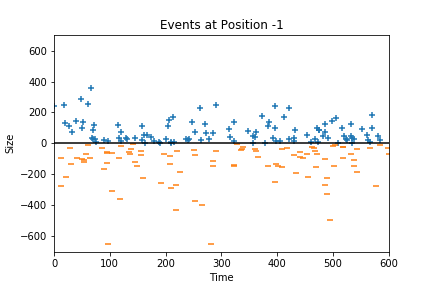
\includegraphics[width=60mm]{Figures/Events/events-1.png}}
{}
\\
\hline
\end{tabular}
\label{fig:bid_events_graphs}
\end{figure}

\begin{figure}
\centering
\caption{Ask Arrivals over $T$ = 600 seconds}
\begin{tabular}{cc}
\hline
\subf{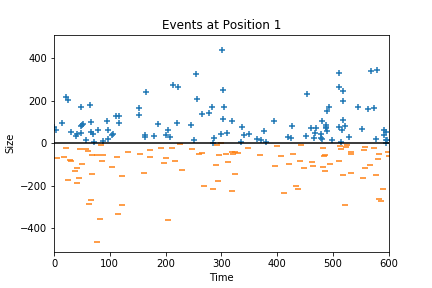
\includegraphics[width=60mm]{Figures/Events/events1.png}}
{}
&
\subf{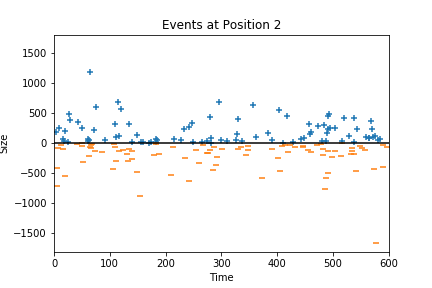
\includegraphics[width=60mm]{Figures/Events/events2.png}}
{}
\\
\subf{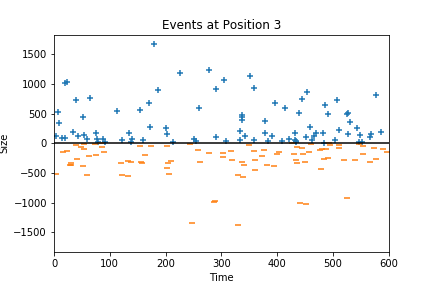
\includegraphics[width=60mm]{Figures/Events/events3.png}}
{}
&
\subf{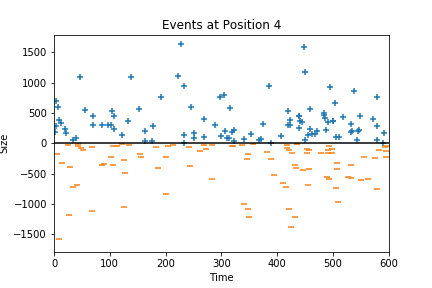
\includegraphics[width=60mm]{Figures/Events/events4.png}}
{}
\\
\subf{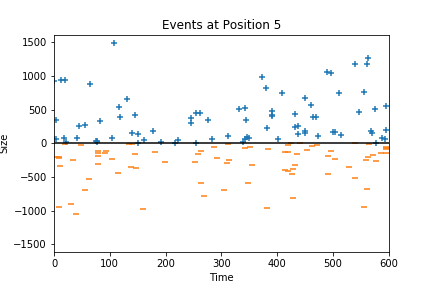
\includegraphics[width=60mm]{Figures/Events/events5.png}}
{}
&
\subf{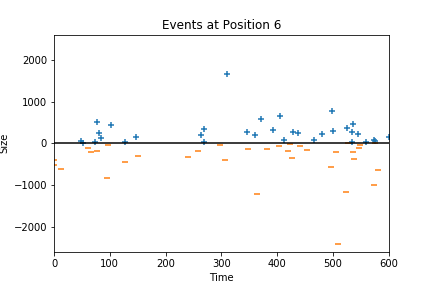
\includegraphics[width=60mm]{Figures/Events/events6.png}}
{}
\\
\subf{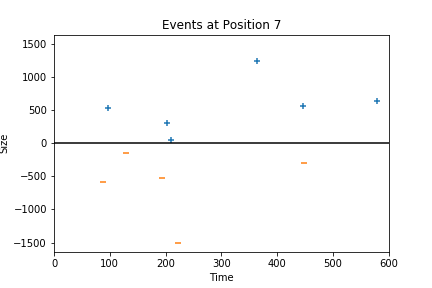
\includegraphics[width=60mm]{Figures/Events/events7.png}}
{}
&
\subf{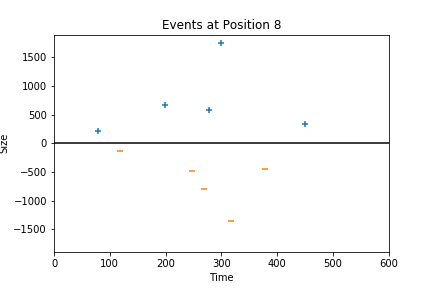
\includegraphics[width=60mm]{Figures/Events/events8.png}}
{}
\\
\subf{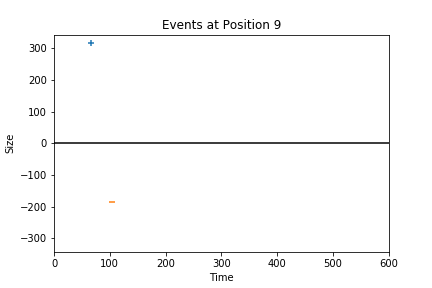
\includegraphics[width=60mm]{Figures/Events/events9.png}}
{}
&
\subf{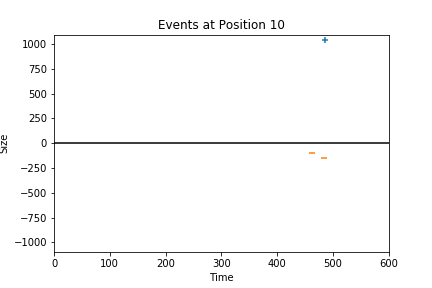
\includegraphics[width=60mm]{Figures/Events/events10.png}}
{}
\\
\hline
\end{tabular}
\label{fig:ask_events_graphs}
\end{figure}

\section{Simulation Algorithm} \label{ch:simulation_algorithm}

The actions of the agent can now be incorporated into the simulation. The agent must buy $V$ units in a time period $T$. It follows a trading schedule $\Omega$, which is a list of market orders of the form $(M,\tau)$ where $M$ is the size of the order and $\tau$ is the time at which it is to be sent. If $V$ units have not been acquired at the end of the time period, the agent makes a market order for the remainder of the inventory to comply with the spirit of the game. LOB events outside of the agent's orders are generated using Algorithm \ref{alg:backwards_simulation}, and the reference price is updated as described in Section \ref{ch:queue_model}. The simulation algorithm is presented below. It returns $\Theta$, a list of executed trades of the form $(p,a,\tau)$ that contains the price, number of units, and time of the trade. The prices are given assuming that there are no trading fees in the exchange.

$$ $$

\begin{algorithm}[H]
\SetAlgoLined
\caption{LOB Simulation: Setup and Input}
Let $p_0$ be the starting reference price \;

Let $L$ be the initial LOB. Let $L_p$ be the volume at price $p$ \;

Let $v$ be the amount of inventory filled \;

Let $\Theta = []$ be the trades executed \;

Let $\Omega$ be the list of market orders in the trading schedule. If $\sum\limits_\Omega{M} < V$, append $(V - \sum\limits_\Omega{M}, T)$ to $\Omega$ \;

Generate $E$ using Algorithm \ref{alg:backwards_simulation} \;

Sort $\Omega$ and $E$ by $\tau$;
\end{algorithm}

\begin{algorithm}[H]
\SetAlgoLined
\caption{LOB Simulation: Recording Executed Trades}
Proceed through $\Omega$ and $E$ in time order. 

\While{$\tau <= T$ and $v < V$} {
    \If {$\text{\upshape event of form}$ $(k,c,\tau)$} {
        Update $L$ and $p_0$ (see Section \ref{ch:queue_model}) \;
    }
    \If {$\text{\upshape order of form}$ $(M,\tau)$} {
        Let $p = p_0 + 0.5$ \;
        \While {$L_p$ = 0} {
            $p \leftarrow p + 1$
        }
        Let $m = M$ \;
        \While {$m > 0$} {
            Let $a = (L_p - m)^+$ \;
            
            $L_p \leftarrow L_p - a$ \;
            
            Append $(p, a, \tau)$ to $\Theta$ \;

            $m \leftarrow m - a$ \;
    
            $p \leftarrow p + 1$ \;
        }
        $v \leftarrow v + M$ \;
        
        Update $p_0$ \;
    }
}

Return $\Theta$ ;
\end{algorithm}

$$ $$

$\Theta$ can then be used to compute the VWAP of the trading schedule. See Listing \ref{code:simulation} for the code written to perform the simulation.